
2025 - 10b

{\bf Chapitre 7 : Espace-temps physique et équations d'Einstein (suite)}
Structure du cadre spatiotemporel
Contenu matériel
Notion d'observateur
Notion d'horloge ; temps propre
Grandeurs physiques relatives à un observateur
Dynamique ; évolution / déploiement dans l'espace-temps
Principe de moindre action ; lagrangien
Intégration sur une variété, jacobien, "forme volume"

Matière champ. Champ EM, tenseur de rang (0,2), tenseur de Faraday
\[
F_{\mu\nu}=\partial_\mu A_\nu-\partial_\nu A_\mu
\]
\[
\delta S=0\qquad-\frac{1}{4}F_{\mu\nu} F^{\mu\nu}
\]
\[
e^{i\frac{S}{\hbar}}\qquad S\to\int \mc{L}
\]
\section{Observateur}
\begin{minipage}[c]{.45\linewidth}
\[
\begin{array}{ c r c l }
 \gamma : & \mb{R} & \to & M \\
  & \lambda & \mapsto & \gamma(\lambda) \\
\end{array}\]
\[
g(\mc{V}_\gamma,\mc{V}_\gamma)<0
\]
\end{minipage}
\hfill
\begin{minipage}[c]{.45\linewidth}
Ligne d'univers de genre temps associé à un choix de base de
T$_{\gamma(\lambda)}$M
\[
\{\vec{e}_{(0)},\vec{e}_{(1)},\vec{e}_{(2)},\vec{e}_{(3)}\}
\]
tel que
\end{minipage}
\[
g(\vec{e}_{(0)},\vec{e}_{(0)})=-1\quad et\quad
g_{ij}g(\vec{e}_{(0)},\vec{e}_{(0)})=\delta_{ij}
\]
\[
g_{\mu\nu}=\eta_{\mu\nu}=\left[
\begin{array}{ c c c c }
 -1 & 0 & 0 & 0 \\
  0 & 1 & 0 & 0 \\
  0 & 0 & 1 & 0 \\
  0 & 0 & 0 & 1 \\
\end{array}\right]
\]
\section{Horloge}
associée à un observateur

mesure une durér entre deux points de la ligne d'un $\gamma_{obs}(\lambda_1)$
et $\gamma_{obs}(\lambda_2)$
\[
L[\gamma_{obs},\lambda_1,\lambda_2]=\int^{\lambda_2}_{\lambda_1}
\sqrt{-g_{(\gamma_{obs}(\lambda))}\big(\mc{V}_{\gamma_{obs}(\lambda)},
\mc{V}_{\gamma_{obs}(\lambda)}\big)}\ d\lambda
\]
durée propre \qquad si $\gamma_{obs}$ est paramétrée par temps propre
\[
g\big(\mc{V}_{\gamma_{obs}(\lambda)},\mc{V}_{\gamma_{obs}(\lambda)}\big)=-1
\]
\[
L[\gamma]=\int d\lambda\sqrt{\mc{V}_{\gamma_{obs},\gamma_{obs}(\lambda)},
\mc{V}_{\gamma_{obs},\gamma_{obs}(\lambda)}}
\]
\section{Grandeurs physiques mesuré/observées}
Les grandeurs physiques fondamentales sont des objet définis de manière intrinsèque, indépendantes d'une carte ou d'un observateur.

$\mc{F}$ champ de tenseurs de Faraday (0,2). En chaque point, F

Dans la base de l'observateur $\gamma_{obs}$ au point p $\in$ M
\[
\{\vec{e}_{(0)}(p),\vec{e}_{(1)}(p),\vec{e}_{(2)}(p),\vec{e}_{(3)}(p)\}
\]
les composantes de $\mc{F}(p)$ sont
\[
F_{ab}=F(\vec{e}_{(a)},\vec{e}_{(b)})
\]
\[
F_{ab}=\left[
\begin{array}{ c c c c }
 0 & E_1 & E_2 & E_3 \\ 
 E_1 & 0 & B_3 & -B_2 \\ 
 E_2 & -B_3 & 0 & B_1 \\ 
 E_3 & B_2 & -B_1 & 0 \\ 
\end{array}
\right]\quad\to\ \vec{f}=q\vec{E}+q\vec{v}\wedge\vec{B}
\]
\[
E^i=F^{0i}\qquad B^i=F_k\varepsilon^{ijk}
\]
\[
g(\mc{V}_{\gamma_{obs}},\mc{V}_{\gamma_{part}}) = g_{\mu\nu}\ \dot
x^\mu_{\gamma_{obs}}\ \dot x^\nu_{\gamma_{part}} = g_{\mu\nu}\ u^\mu v^\nu
\]
facteur de Lorentz
\[
\vec{v} = \mc{V}_{\gamma_{part}}\vec e_{i}
\]
énergie de la particule du point de vue de l'observateur
\[
E=-g\big(m\mc{V}_{\gamma_{part}},\mc{V}_{\gamma_{obs}}\big)
\]
\[
\Delta A^M-\frac{1}{c^2}\frac{\partial^2A^M}{\partial t^2}=0
\qquad \Delta \vec E-\frac{1}{c^2}\frac{\partial^2\vec E}{\partial t^2}=0
\]
\[\]
\[\]
\section{Dynamique}
Principe de moindre action
\[
\delta S=0\qquad S\int^{t_2}_{t_1}L(q,\dot q)dt
\]
équation d'Euler-Lagrange
\[
\frac{d}{dt}\big(\frac{\partial L}{\partial\dot q}\big)-
\frac{\partial L}{\partial q}=0
\]
particule ponctuelle
\[
S[\gamma]=-mc\int d\tau=-mc\int^{\lambda_2}_{\lambda_1}\sqrt{g_{\mu\nu}
\ \dot x^\mu_\gamma\ \dot x^\nu_\gamma}\ d\lambda
\]
\[
\delta S=0\quad \to\ \ddot x^i\gamma +\Gamma^i_{jk}
\ \dot x^j_\gamma\ \dot x^k_\gamma=0
\]
\[
S[\gamma_1,\gamma_2]=S_{part\ 1}[\gamma_1]
+S_{part\ 2}[\gamma_2]S_{int}[\gamma_1,\gamma_2]
\]

\[
\delta S \ \ / \ \ \delta\gamma_1\ \ \delta\gamma_2
\]
\[
S[\gamma]=-mc\int dx\int d\lambda\sqrt{-g_{\mu\nu}\ \dot x^\mu_\gamma
\ \dot x^\nu_\gamma}\ \delta(x-x_\gamma(\lambda))
\]

f dérivable
\begin{minipage}[c]{.45\linewidth}
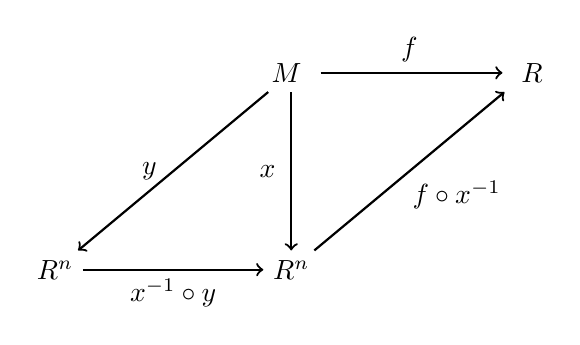
\begin{tikzpicture}
\def\largeur{3} \def\hauteur{2.5} \def\decalage{0.3} \node (A) at (0,0) {$M\ $};
\node (B) at (\largeur,0) {$\ \mb{R}$};
\node (C) at (-\largeur,-\hauteur) {$\mb{R}^n$};
\node (D) at (0,-\hauteur) {$\mb{R}^n$};
%
\node (I) at (0.5*\largeur ,\decalage) {$f$};
\node (G) at (-0.5*\largeur-\decalage ,-0.5*\hauteur) {$y$};
\node (H) at (-\decalage ,-0.5*\hauteur) {$x$};
\node (E) at (-0.5*\largeur ,-\hauteur-\decalage){$x^{-1}\circ y$};
\node (F) at (0.5*\largeur+2*\decalage ,-0.5*\hauteur-\decalage){$f\circ x^{-1}$};
\draw[thick,->] (A)--(B);\draw[thick,->] (A)--(C);\draw[thick,->] (A)--(D);
\draw[thick,->] (C)--(D);\draw[thick,->] (D)--(B);\end{tikzpicture}
\end{minipage}
\hfill
\begin{minipage}[c]{.45\linewidth}
\[
\frac{\partial f}{\partial x^i}=\partial_i(f\circ x^{-1})
\]
\[
\int_\mc{U}f=\int_{x}(f\circ x^{-1})dx^1...dx^n
\]
\end{minipage}


\[
\]
\[
\]
\[
\]
\[
\]
\[
\]
